\section{Regular expressions and FSA}

Take a two-letter alphabet $\Sigma=\{a,b\}$. 
Consider the nondeterministic automaton $A$ over $\Sigma$ below, which has spontaneous transitions ($\varepsilon$-transitions): 
\begin{figure}[H]
    \centering
    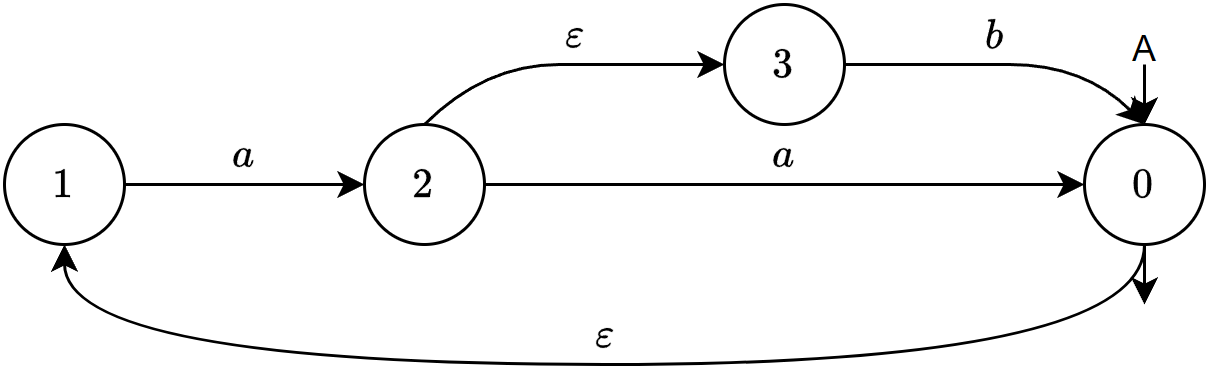
\includegraphics[width=0.5\linewidth]{images/FSA1a.png}
\end{figure}
And consider also the regular expression $R$ over $\Sigma$ below:
\[R=\left( aa|ab|ba \right)^{*}\]
Answer the following questions:
\begin{enumerate}
    \item Find all the valid strings of language $L(A)$ that have a length less or equal than four. 
        Do the same for language $L(R)$, too.
    \item By using the back propagation method, eliminate the spontaneous transitions of automaton $A$ and obtain an equivalent deterministic automaton $A_1$ without spontaneous transitions. 
        Clean and minimize automaton $A_1$, if necessary. 
        Test automaton $A_1$ with the valid short strings found at point one for automaton $A$. 
    \item By using the Berry-Sethi method, obtain a deterministic automaton $A_2$ equivalent to the regular expression $R$. 
        Minimize automaton $A_2$, if necessary. 
        Test automaton $A_2$ with the valid short strings found at point one for expression $R$.
    \item Say if language $L(R)$ is local or not, and shortly justify your answer.
    \item By using a systematic method of your choice, obtain a deterministic automaton $A_3$ for the difference language $L_D=L(R)-L(A)$, i.e., $L(R) \cap \overline{L(A)}$, which contains the strings generated by $R$ that are not recognized by $A$. 
        Then test automaton $A_3$: by examining (only) the strings of length 4 found at point one, find in alphabetical order the first two strings $x$ and $y$ such that $x \in L_D$ and $y \notin L_D$, and show that $x \in L(A_3)$ and $y \notin L(A_3)$.
\end{enumerate}

\paragraph*{Solution}
\begin{enumerate}
    \item The strings in the language $L(A)$ are $\varepsilon$, $aa$, $ab$, $aaaa$, $aaab$, $abaa$, and $abab$. 
        The strings in the language $L(R)$ are $\varepsilon$, $aa$, $ab$, $ba$, $aaaa$, $aaab$, $aaba$, $abaa$, $abab$, $abba$, $baaa$, $baab$, and $baba$. 
    \item The backpropagation method involves starting from the arriving state of an $\varepsilon$ transition, eliminating the spontaneous transition, and backpropagating the transition exiting from the state. 
        In this case, the resulting automaton is:
        \begin{figure}[H]
            \centering
            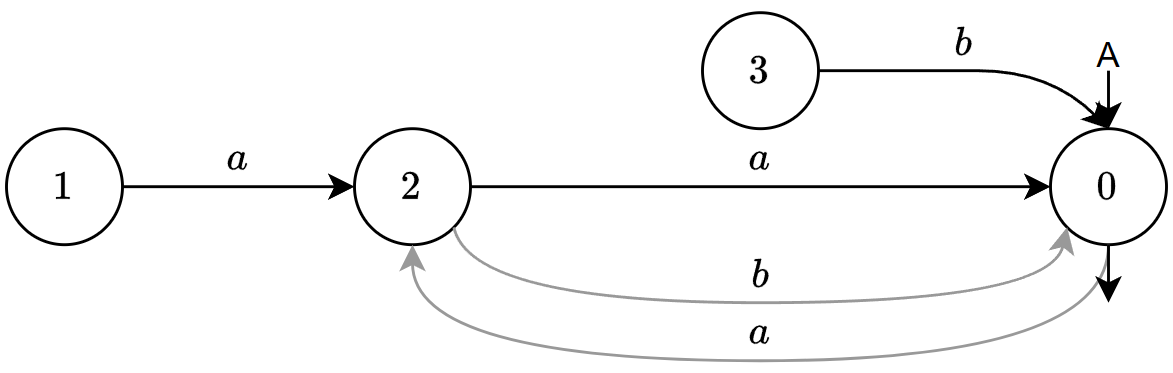
\includegraphics[width=0.5\linewidth]{images/FSA2a.png}
        \end{figure}
        After that we can remove the useless states and rename the remaining ones. 
        \begin{figure}[H]
            \centering
            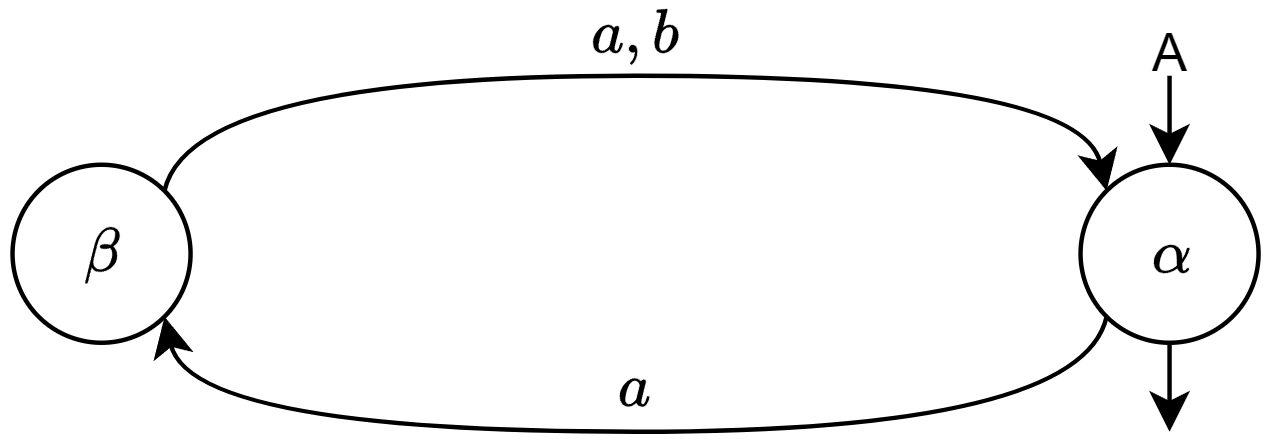
\includegraphics[width=0.5\linewidth]{images/FSA3a.png}
        \end{figure}
        The states are undistinguishable, so the automaton is the minimal one, and it is the same as the initial one. 
    \item Firstly, we enumerate the symbols $R_{\#}=\left( a_1a_2|a_3b_4|b_5a_6 \right)^{*}\dashv$. 
        We construct the following support table: 
        \begin{table}[H]
            \centering
            \begin{tabular}{cc}
            Initials                       & $a_1a_3a_5\dashv$              \\ \hline
            \multicolumn{1}{c|}{Terminals} & Followers                      \\
            \multicolumn{1}{c|}{$a_1$}     & $a_2$                          \\
            \multicolumn{1}{c|}{$a_2$}     & $a_1a_3a_5\dashv$              \\
            \multicolumn{1}{c|}{$a_3$}     & $b_4$                          \\
            \multicolumn{1}{c|}{$b_4$}     & $a_1a_3a_5\dashv$              \\
            \multicolumn{1}{c|}{$b_5$}     & $a_6$                          \\
            \multicolumn{1}{c|}{$a_6$}     & $a_1a_3a_5\dashv$ 
            \end{tabular}
        \end{table}
        The resulting automaton is already minimal:
        \begin{figure}[H]
            \centering
            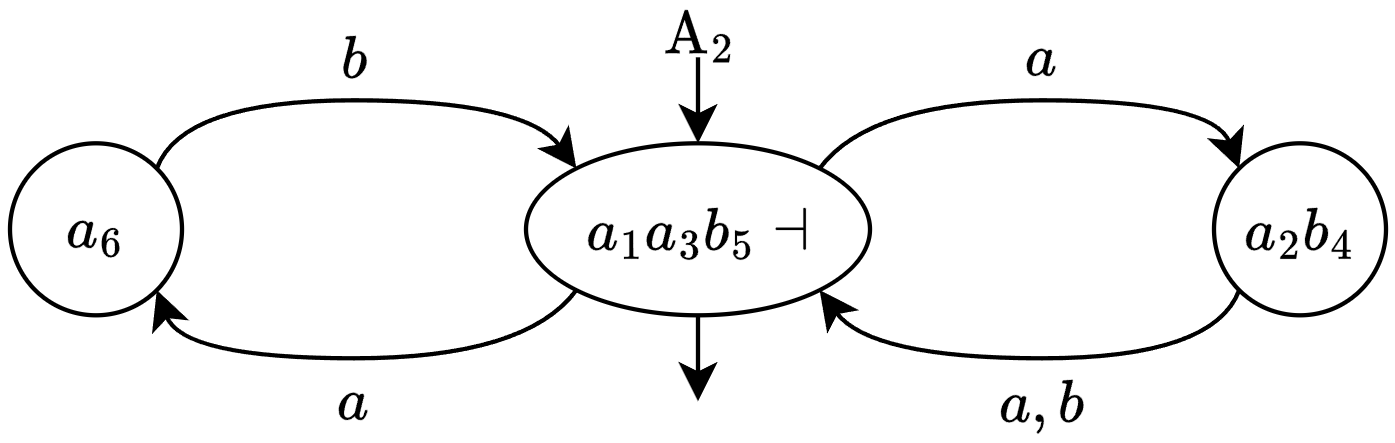
\includegraphics[width=0.6\linewidth]{images/FSA4a.png}
        \end{figure} 
    \item The language is not local. 
        Although automaton $A_2$ is minimal, it is not local. 
        The minimal automaton of a local language is necessarily local.
    \item The language $L_D=L(R)-L(A)=L(R) \cup \overline{L(A)}$. 
        To find the complement of automaton $A$, we switch final and non-final states and add an error state $\eta$.
        This results in:
        \begin{figure}[H]
            \centering
            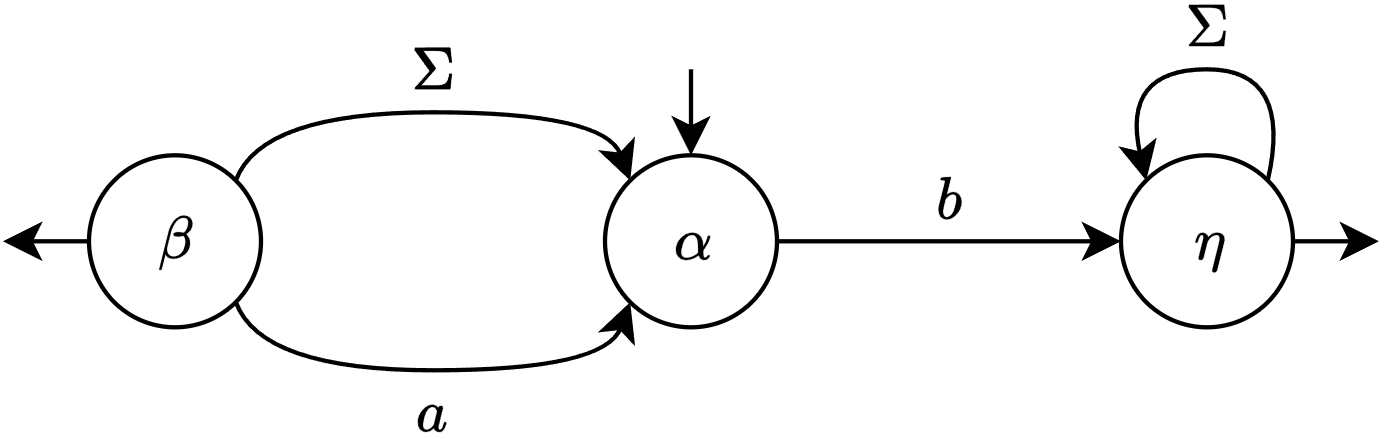
\includegraphics[width=0.5\linewidth]{images/FSA5a.png}
        \end{figure}
        Rewriting automaton $A_2$:
        \begin{figure}[H]
            \centering
            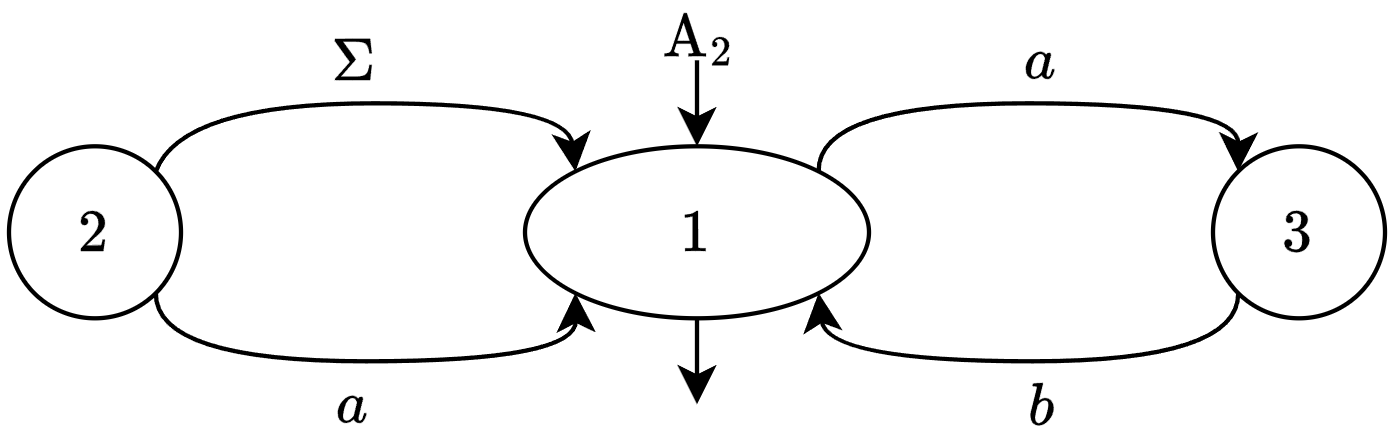
\includegraphics[width=0.5\linewidth]{images/FSA6a.png}
        \end{figure}
        By connecting states with both transitions, we obtain:
        \begin{figure}[H]
            \centering
            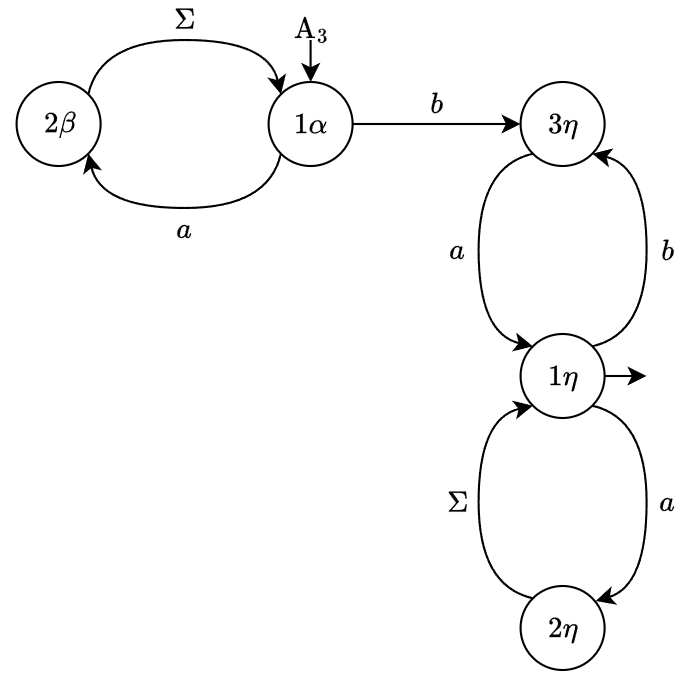
\includegraphics[width=0.5\linewidth]{images/FSA7a.png}
        \end{figure}
        Automaton $A_3$ has only five states, is deterministic, and is clean.
        While it may not be minimal, it passes a test where alphabetically listing the length-4 strings of language $L(R)$ and $L(A)$ reveals that $A_3$ correctly recognizes certain strings.
\end{enumerate}